\documentclass{standalone}
\usepackage{tikz}
\usetikzlibrary{shapes.geometric}
\begin{document}

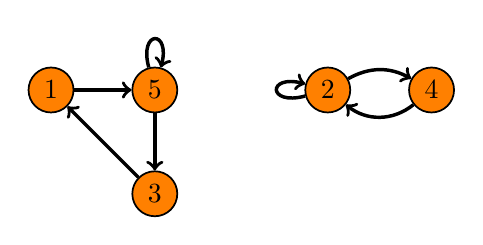
\begin{tikzpicture}
[every node/.style={inner sep=0pt}]
\node (1) [circle, minimum size=16.25pt, fill=orange, line width=0.625pt, draw=black] at (37.5pt, -37.5pt) {\textcolor{black}{1}};
\node (2) [circle, minimum size=16.25pt, fill=orange, line width=0.625pt, draw=black] at (137.5pt, -37.5pt) {\textcolor{black}{2}};
\node (3) [circle, minimum size=16.25pt, fill=orange, line width=0.625pt, draw=black] at (75.0pt, -75.0pt) {\textcolor{black}{3}};
\node (4) [circle, minimum size=16.25pt, fill=orange, line width=0.625pt, draw=black] at (175.0pt, -37.5pt) {\textcolor{black}{4}};
\node (5) [circle, minimum size=16.25pt, fill=orange, line width=0.625pt, draw=black] at (75.0pt, -37.5pt) {\textcolor{black}{5}};
\draw [line width=1.25, ->, color=black] (1) to  (5);
\draw [line width=1.25, ->, color=black] (5) to  (3);
\draw [line width=1.25, ->, color=black] (3) to  (1);
\draw [line width=1.25, ->, color=black, loop above] (5) to (5);
\draw [line width=1.25, ->, color=black, loop left] (2) to (2);
\draw [line width=1.25, ->, color=black] (2) to  [in=151, out=29] (4);
\draw [line width=1.25, ->, color=black] (4) to  [in=321, out=219] (2);
\end{tikzpicture}

\end{document}
